Fino ad ora abbiamo sempre supposto di essere in grado di misurare gli oggetti di cui stiamo parlando: ad esempio le particelle $\alpha$, gli elettroni e positroni nel decadimeto $\beta$ e $\gamma$ prodotti da transizioni nucleari, annichilazione di $e^+e^-$, cattura elettronica. Abbiamo visto anche che, in alcuni casi, possiamo rivelare particelle tramite interazioni che producono particelle visibili: $n$ attraverso il rinculo nucleare (Chadwick), e il $\nu$ attraverso il decadimento $\beta$ inverso (Reines e Cowan). In generale tutti i processi di rivelazione si basano su interazioni di una particellam in cui parte dell'energia della particella viene trasferita ad un materiale. Alla fine questa energia si trasformerà in calore (come abbiamo visto in fusione e fissione). La rivelazione sfrutta un fenomeno transiente pricma che avvenga la termalizzazione. Eccezione: i bolometri che misurano l'aumento di temperatura ad esempio l'esperimento CUORE al gran sasso in cui si lavora a temperature davvero basse (si parla del metrocubo più freddo dell'universo). Il processo principale è l'\textbf{interazione di particelle cariche} con gli elettroni del materiale attraversato: perdita di energia di particelle "veloci", range e picco di Bragg. Per particelle ultra-relativistiche entra in gioco la perdita di energia per radiazione. Dovuta all'accelerazione che la particella sente nel materiale. Quantità caratteristiche: lunghezza di interazione $X_0$.

Per \textbf{particelle neutre} si sfrutta il trasferimento di energia a particelle cariche: abbiamo già parlato diffusamente di diffusione elastica per $n$, interazione di fotoni con la materia: effetto fotoelettricom effetto Compton, produzione di coppie. Ad altissime energie possono prodursi fenomenti di grande estensione: conversione di energia cinetica in massa (vengono chiamate sciami di particelle).


Osservazione di un segnale prodotto dal deposito di energia di particelle cariche (questi conti si riciclano anche dal punto di vista medico): sua particelle primarie, che "entrano nel rivelatore", sia particelle secondarie, prodotte dalle interazioni con il rivelatore. 
\subsection{Perdita di energia per collisione}
La perdita di energia da parte di una particella carica è dominata dall'interazione con gli elettroni del mezzo. Assumiamo che la particella carica sia \textbf{veloce} e \textbf{pesante}: supponiamo che l'eletrone durante l'interazione sia fermo e che nella singola interazione la particella non venga deviata apprezzabilmente. Un elettrone a distanza $b$ dalla particella, sente il campo elettrico della particella. Vediamo quanta energia viene guadagnata dall'elettrone. Durante il tempo di interazione l'elettrone riceve un impulso:
\begin{equation*}
    \Delta P=\int F dt=\int (-e)E dt
\end{equation*}
L'impulso totale è trasverso in quando le componenti lungo l'asse di percorrenza si cancellano. Dopo l'interazione l'elettrone ha una energia cinetica:
\begin{equation*}
    T=\frac{\Delta P^2}{2m_e}
\end{equation*}
Fornita dalla particella in movimento. Per calcolare il momento trasferito è comodo mettersi nel sistema di riferimento di quiete della particella. Siccuome le componenti trasverse non contano:
\begin{equation*}
    \Delta P=\int (-e)E_\perp dt=e\int E_\perp \frac{dt}{dz}dz=\frac{e}{v}\int E_\perp dz
\end{equation*}
Moltiplicando entrambi i membri per $2\pi b$:
\begin{equation*}
    2\pi b \Delta P=\frac{e}{v}\int E_\perp dzbd\phi=\frac{e}{v}\Phi(E)=\frac{e}{v}\frac{ze}{\varepsilon_0}
\end{equation*}
dove la zeta nella seconda frazione rappresenza la carica. Quindi:
\begin{equation*}
    \Delta P=\frac{ze^2}{2\pi\varepsilon_0}\frac{1}{vb}=2\alpha z\frac{\hbar c}{vb}=2\alpha z \frac{\hbar}{\beta b}
\end{equation*}
L'energia trasferita all'elettrone è quindi:
\begin{equation*}
    \Delta E=\frac{\Delta P^2}{2m_e}=2z^2\alpha^2\frac{\hbar^2}{m_e\beta^2b^2}
\end{equation*}
Il problema è che abbiamo ancora dentro il parametro di impatto. Possiamo chiarire meglio l'approssimazione di particella veloce e pesante: nell'urto la particella subisce una perdita di energia $\Delta E$ ed una deviazione $\Delta \theta=\Delta P/P=\Delta P/M\beta c$. Infatti i risultati sono validi se:
\begin{equation*}
    \frac{\Delta P}{P}=\frac{ze^2}{2\pi\varepsilon_0}\frac{1}{Mv^2b}\frac{1}{\frac{1}{2}Mv^2}<<1 \text{ e } \Delta E<<\frac{1}{2}Mv^2
\end{equation*}
Percorrendo uno spazio $dx$, la particella incontra un numero di elettroni a distanza b: $2\pi bdbdxn_e$ dove $n_e=Z\frac{N_A}{A}\rho$ è la densità di elettroni. La perdita di energia per unità di lunghezza è data dall'integrale sui parametri di impatto:
\begin{equation*}
    \frac{dE}{dx}=\int_{b_{min}}^{b_{max}}2\pi bdbn_e2z^2\alpha^2\frac{\hbar^2}{m_e\beta^2b^2}=\frac{4\pi z^2\alpha^2\hbar^2 n_e}{m_e\beta^2}\int_{b_{min}}^{b_{max}}db\frac{1}{b}=\frac{4\pi z^2\alpha^2\hbar^2}{m_e\beta^2}Z\frac{N_A}{A}\rho\ln{\frac{b_{max}}{b_{min}}}
\end{equation*}
Il punto critico sono gli estremi di integrazione $b_{min}$ e $b_{max}$. In realtà corrispondono alle energie trasferite $E_{max}$ e $E_{min}$ rispettivamente visto che l'energia è inversamente proporzionale al quadrato del parametro di impatto:
\begin{equation*}
    E_{max}=2z^2\alpha^2\frac{\hbar^2}{m_e\beta^2b_{min}^2} \qquad E_{min}=2z^2\alpha^2\frac{\hbar^2}{m_e\beta^2b_{max}^2}
\end{equation*}
\begin{equation*}
    \frac{dE}{dx}=\frac{4\pi r_e^2m_ec^2}{\beta^2}\frac{z^2ZN_A\rho}{A}\frac{1}{2}\ln{\frac{E_{max}}{E_{min}}}
\end{equation*}
dove $r_e$ è il raggio classico dell'elettrone: $r_e=\alpha\frac{\hbar}{m_ec}$. DIversi testi usano diverse approssimazioni/stime di tali parametri di impatto ed energie. Tenendo le cose più semplici possibili l'energia massima è l'energia massima trasferibile in un urto con l'elettrone. $E_{max}=T_{max}$. 
\begin{equation*}
    E_{\max }=T_{\max }=\frac{2 \gamma^2 \beta^2 m_e c^2}{1+2 \gamma m_e / M+\left(m_e / M\right)^2}
\end{equation*}
Mentre l'energia minima è l'energia media di eccitazione degli elettroni più esterni. Facendo un calcolo completo di Bethe-Bloch:
\begin{equation*}
    \frac{d E}{d x}=4 \pi r_e^2 m_e c^2 \frac{z^2 Z N_A \rho}{A} \frac{1}{\beta^2}\left[\frac{1}{2} \ln \frac{2 \gamma^2 \beta^2 m_e c^2 T_{\max }}{\bar{I}^2}-\beta^2-\frac{\delta(\gamma \beta)}{2}\right] 
\end{equation*}
 %IMMAGINE bb
\begin{figure}[htp!]
  \centering
  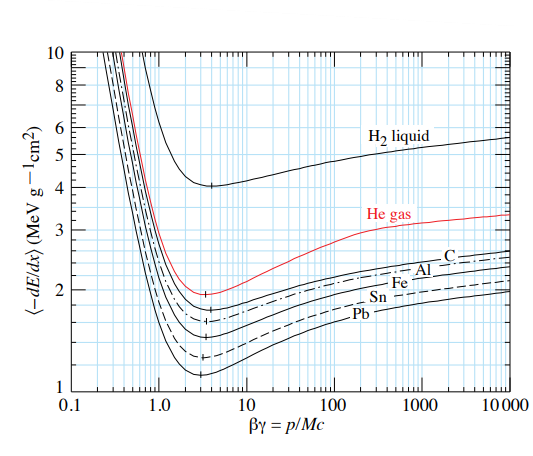
\includegraphics[scale=0.7]{Lezione14/bb.png} 
\end{figure}
La cosa interessante è che non entra mai la massa della particella incidente, ma solo da $\beta\gamma$. Nella parte bassa va come $1/\beta^2$ poi ha una risalita detta risalirta relativistica che va come $\ln{\gamma}$. Successivamente questo andamento presenta un minimo per stati della materia diversi e per elementi diversi. Tutti sono con un minimo più o meno nello stesso punto $\gamma\beta\sim 3$. Ad esempio voglio mandare protoni contro del piombo e voglio capire quanto piombo mi serve per fermarli. Faccio il conto supponendo che sia al minimo di ionizzazione. Quindi sono nell'ipotesi in cui i miei protoni perdono il minimo dell'energia. Poi c'è un effetto $\delta$ dovuta alla polarizzazione del mezzo.

Consideriamo il prefattore:
\begin{equation*}
    4\pi r_e^2m_ec^2N_A=0.307\,MeV\,cm^2\,mol^{-1}
\end{equation*}
Il materiale entra con $\frac{Z}{A}\sim 0.5\,mol/g$. Il grosso della dipendenza dal materiale viene dalla densità. Conviene definire lo spessore in termidi di densità superficiale $x\rho$.
\begin{equation*}
    \frac{dE}{d(x\rho)}=4 \pi r_e^2 m_e c^2 N_A\frac{Z}{A}\frac{z^2}{\beta^2}\left[\frac{1}{2} \ln \frac{2 \gamma^2 \beta^2 m_e c^2 T_{\max }}{\bar{I}^2}-\beta^2-\frac{\delta(\gamma \beta)}{2}\right] 
\end{equation*}
L'unità di misura sarà quindi: $MeV/(g/cm^2)$. Poco dipendente dal materiale:
\begin{equation*}
     4\pi r_e^2m_ec^2N_A\frac{Z}{A}\approx0.15\,\frac{MeV}{g/cm^{2}}
\end{equation*}
al minimo (per particelle unitarie altrimenti bisogna calolare per uno $z^2$):
\begin{equation*}
    \frac{dE}{d(x\rho)}\approx1.5\,\frac{MeV}{g/cm^2}
\end{equation*}
Se una particella è al minimo di ionizzazione (cosa che accade spesso) in prima approssimazione la particelle perde questa quantità di energia.
\subsection{Fluttuazioi della perdita di energia}
Il processo di interazione degli elettroni è un processo statistico. Deviazione angolare: \textbf{scattering multiplo}, nel singolo $\Delta \theta=\Delta P/P$. Siccome gli elettroni sono distribuiti in tutte le direzioni $\langle \Delta\theta\rangle=0$, ma con una varianza $\langle \Delta\theta^2\rangle>0$. L'effetto comulatico su tanti urti è una deflessione con una deviazione:
\begin{equation*}
    \theta_{rms}\approx\frac{13.6\,MeV}{\beta p c } z\sqrt{\frac{L}{X_0}}
\end{equation*}
Questo è importante perchè dal punto di vista geometrico facciamo finta che voglio mettere in cascata due rivelatori. A questo punto voglio capire quanto deve essere grande in modo tale da non perdere particelle. La perdita di energia ha due processi che corrispondono a tante collisioni a piccolo $\Delta E$ mentre poche collisioni con grande $\Delta E$. Queste ultime inducono fluttuazioni nella pertita di energia:
%IMMAGINE r1 r2
\begin{figure}[htp!]
  \centering
  
\includegraphics[scale=0.8]{Lezione14/r1.png}
  
\includegraphics[scale=0.5]{Lezione14/r2.png} 
\end{figure}
Essendo un conto medio ci sarà una deviazione standard.
\subsection{Range e picco di Bragg}
Abbiamo detto che la perdita di energia per ionizzazione è funzione solo della velocità della particella (e del materiale):
\begin{equation*}
    -\frac{dE}{dz}=z^2f(\beta)
\end{equation*}
Possiamo invertire la formula e scrivere:
\begin{equation*}
    dx=-\frac{dE}{z^2f(\beta)}
\end{equation*}
Inoltre, dal momento che $E=m\gamma\to dE=md\gamma$. Possiamo pertanto calcolare la distanza percorsa da una particella prima di fermarsi (\textbf{range}):
\begin{equation*}
    R(\gamma\beta)=\int_0^Rdx
\end{equation*}
Arrivando al risultato:
\begin{equation*}
    R(E)=\frac{m}{z^2}F\left(\frac{E}{m},Z\right)
\end{equation*}
%IMMAGINE d1 d2
\begin{figure}[htp!]
  \centering
  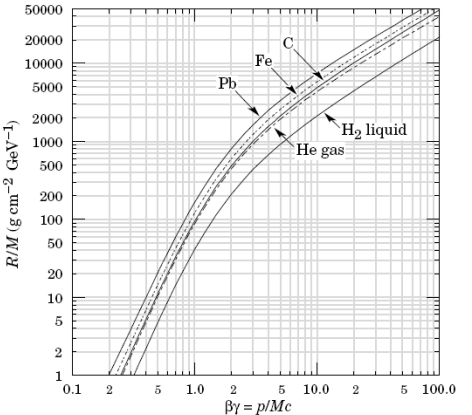
\includegraphics[scale=0.6]{Lezione14/d1.png}
  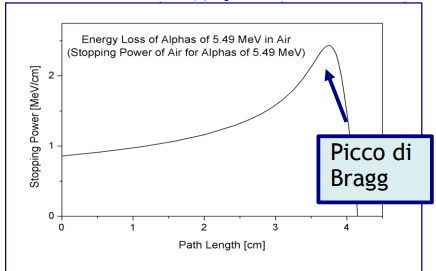
\includegraphics[scale=0.8]{Lezione14/d2.png} 
\end{figure}
La cosa interessante è che più o meno per tutti i materiali si comporta allo stesso modo. Visto che $f(\beta)\sim1/\beta^2$ nel pezzo iniziale. Allora significa che dal gradico posso capire che se la particella si trova all'inzio e si sposta anche solo di poco, nel grafico si sposta di molto verso l'alto. Significa che l'interazione dopo perderà ancora più energia. Quindi una particella che si trova al minimo di ionizzazione nelle prime collisioni perderà poca energia mentre più si avvicina verso sinistra più l'energia persa aumenta. Nel picco alla fine smette di valere l'approssimazione. Il crollo dopo il picco è perchè la particella si è fermata dopo $4\,cm$. Questo viene chiamato il Picco di Bragg. Funzionamento dell'adroterapia. Il grafico della particella del fotone è praticamente piatta. Quindi se voglio curare il tumore con dei raggi X oltre a irradiare il tumore irradierò anche tutti gli altri tessuti in egual modo con danni. Se si usano delle particelle e si sanno calibrare bene si può fare in modo che il picco finisca esattamente dove è il tumore. In questo modo i tessuti sani ricevono solo una piccola quantità di energia. 
\subsection{Perdita di energia per radiazione}
Anche se ricavata per particelle "pesanti", la forma di Bethe-Bloch funziona ragionevolmente anche per elettroni. Però ci sono alcune differenze. Nell'urto è possibile trasferire una grande frazione dell'energia ad altri elettroni. Ci possono essere grandi accelerazioni nello scattering su nuclei e le particelle accelerate emettono radiazione. \textbf{Bremsstrahlung}: radiazione di frenamento. Ora ne stiamo parlando per gli elettroni perchè è il caso più evidente. Ma ad energie abbastanza alte (tutto dipende da $\beta\gamma$) c'è radiazione di frenamento. Fenomenologicamente si osserva che l'emissione di energia è proporzionale all'energia stessa:
\begin{equation*}
    \frac{dE}{dx}=\frac{E}{X_0}
\end{equation*}
Il coefficiente di proporzionalità $X_0$ prende il nome di \textbf{lunghezza di radiazione}. Questo è il processo usato nei dubi di raggi X. Prendo degli elettroni li faccio schiantare da qualche parte ed in questo modo emettono raggi X.
\subsection{Lunghezza di radiazione}
La lunghezza di radiazione di radiazione di può esprimere come:
\begin{equation*}
    X_0=\frac{716.4\,A}{Z(Z+1)\ln{[287/\sqrt{Z}]}}\,\frac{g}{cm^2}
\end{equation*}
Il termine $Z(Z+1)$ teine conto sia dell'irraggiamento su nucleo che su elettroni. Entra in numerosi altri processi elettromagnetici: scattering multipli e produzione di coppie. Ovviamente opera in competizione con la perdita di energia per collisione.
\begin{equation*}
    \frac{dE}{dx}=-\left\langle\frac{dE}{dx}\right\rangle_{coll}-\frac{E}{X_0}
\end{equation*}
La perdita di energia per collisione è indipendente dal materiale e varia come $\ln{E}$. La zona di più alta energia c'è competizione a bassa energia domina la perdina di energia per bremsstrahulung che dipende da $\sim Z$ e aumenta con $E$.
Quindi si definisce l'\textbf{energia critica} per cui
\begin{equation*}
    \left\langle\frac{dE}{dx}\right\rangle_{coll}=\frac{E}{X_0} \qquad E_c=X_0 \left\langle\frac{dE}{dx}\right\rangle_{coll}
\end{equation*}
Per $E<E_c$ prevale la collisione, per $E>E_c$ prevale la radiazione. Quindi se abbiamo elettroni di energia molto elevata possiamo dimenticarci della Bethe-Bloch perchè la perdita di energia sarà solo per radiazione. Vicino all'energia critica entrambe le perdite di energia hanno un buon contributo e devo considerarle entrambe. Questo è un grafico che riassume la \textbf{perdita di energia di particelle cariche}:
 %IMMAGINE riss
\begin{figure}[htp!]
  \centering
  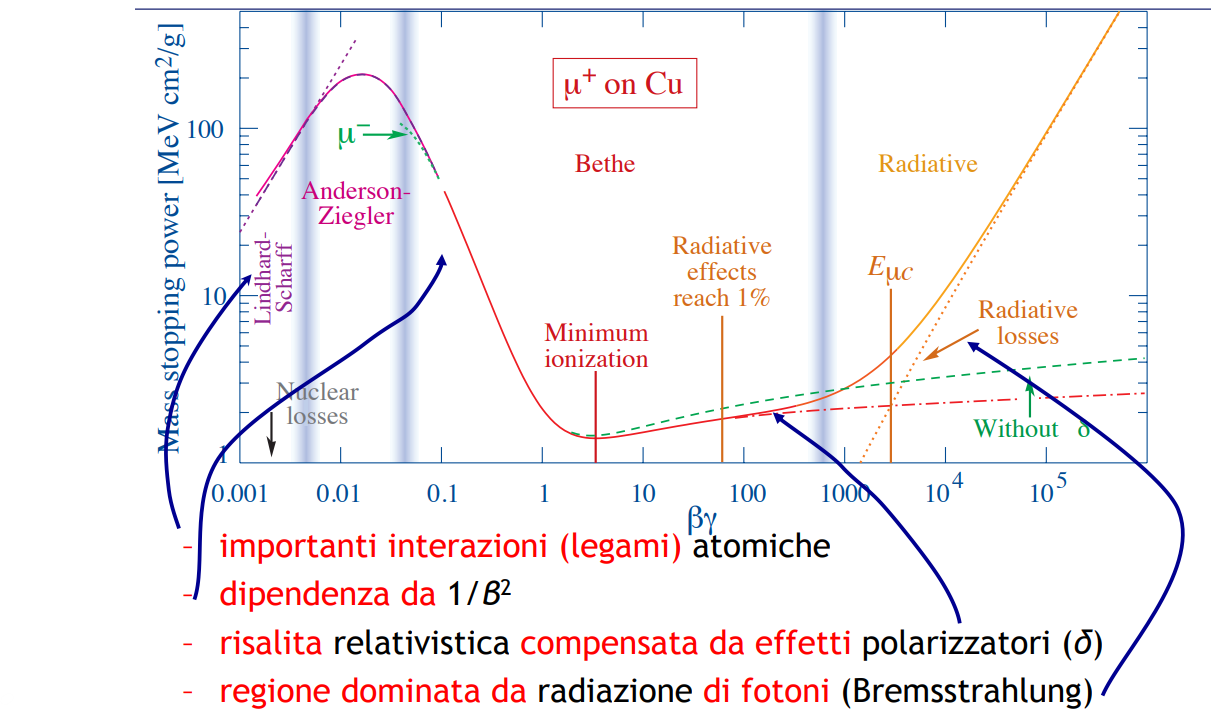
\includegraphics[scale=0.5]{Lezione14/riss.png} 
\end{figure}
\subsection{Interazioni di fotoni}
L'interazione dei fotoni con la materia provoca sostanzialmente 3 tipi di fenomeni: \textbf{effetto fotoelettico} se si bersaglia un pezzo di metallo con della luce vengono fuori degli elettroni in modo quantizzato. Funziona appunto che arriva un fotone da energia ad un elettrone e lo strappa dal nucleo. \textbf{effetto Compton} o \textbf{diffusione da parte degli elettroni} arriva un fotone interagisce con un elettrone (libero), interagisce contro l'elettrone e gli trasferisce parte dell'energia. Infine a energie sufficientemente alte il fotone ha abbastanza energia per produrre materia: \textbf{produzione di coppie elettrone-positrone}. La materia viene prodotta in modo da bilanciare matieria e anti-materia. 

Sono 3 processi molto complessi e diversi tra di loro. L'importanza relativa dei 3 processi dipende sostanzialmente dall'energia del fotone e dal numero atomico del materiale assorbitore (quindi la carica e quindi la Z del materiale). Anche nel caso dei fotoni si ha una \textbf{legge di assorbimento} di tipo esponenziale:
\begin{equation*}
    N(x)=N_0\text{exp}[-\mu x]
\end{equation*}
dove 
\begin{equation*}
    \mu=\frac{\rho}{A}N_A\sigma=\frac{\rho}{A}N_A(\sigma_{p.e.}+\sigma_{Compton}+\sigma_{Coppie})
\end{equation*}
Dove dipendono tutte da $(E_\gamma, Z)$:
 %IMMAGINE k
\begin{figure}[htp!]
  \centering
  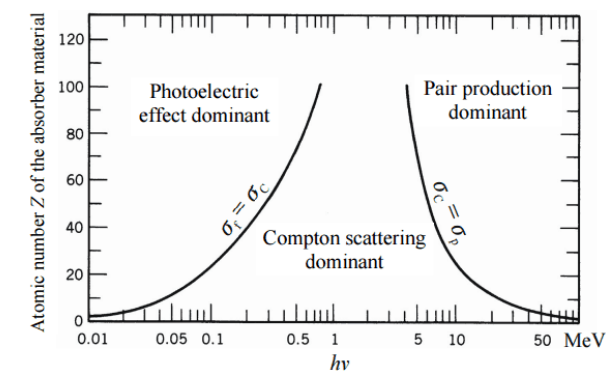
\includegraphics[scale=0.6]{Lezione14/k.png} 
\end{figure}
A circa $1\,MeV$ per qualsiasi $Z$ domina Compton, e così via. Questo è ancora una volta di processi che dominano su altri quindi ci sono situazioni in cui devo tener conto dei vari processi e quindi non vale trascurare.
\subsection{Effetto fotoelettrico}
In questo processo il fotone riesce a trasferire all'elettrone atomico una quantità di energia sufficiente a ionizzarlo, ovviamente questo processo ha una soglia (che dipende da atomo a atomo). L'energia di legame degli elettroni in unatomo complesso ha diversi valori discreti legati alla struttura a shell:
%IMMAGINE ft1 ft2
\begin{figure}[htp!]
  \centering
  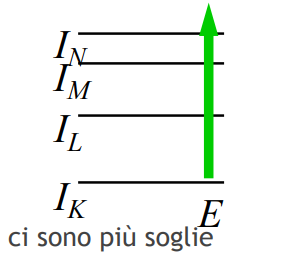
\includegraphics[scale=0.7]{Lezione14/ft1.png}
  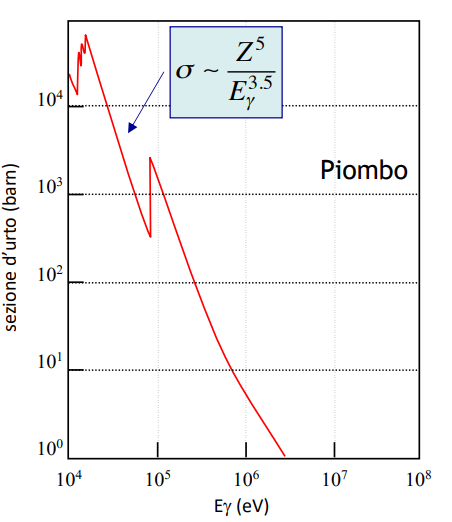
\includegraphics[scale=0.6]{Lezione14/ft2.png} 
\end{figure}
Il processo è possibile solo se l'energia del fotone è maggiore dell'energia della shell $E_\gamma>I_{K,L,\ldots}$. L'elettrone emesso ha un'energia $T_e=E_\gamma -I_X$
\subsection{Scattering Compton}
[slide e appunti]
\subsection{Produzione di copie}
Conversione dell'energia di un fotone in coppia elettrone-positrone. Interazione $\gamma$-nulceo, o $\gamma-e$ (non disponibile nel vuoto per conservare energia-momento). Esiste un'energia di soglia su nucleo:
\begin{equation*}
    \sqrt{s}>2m_ec^2+m(A,Z)c^2
\end{equation*}
o su elettrone: $\sqrt{s}>3m_ec^2$. Al di sopra della soglia la sezione d'urto rapidamente satura ad un valore costante. Anche in questo caso il coefficiente di assorbimento è legato alla lunghezza di radiazione $X_0$.
\begin{equation*}
    \mu_{coppie}=\frac{7}{9}\frac{1}{X_0}
\end{equation*}
\subsection{Interazioni di fotoni}
 %IMMAGINE h
\begin{figure}[htp!]
  \centering
  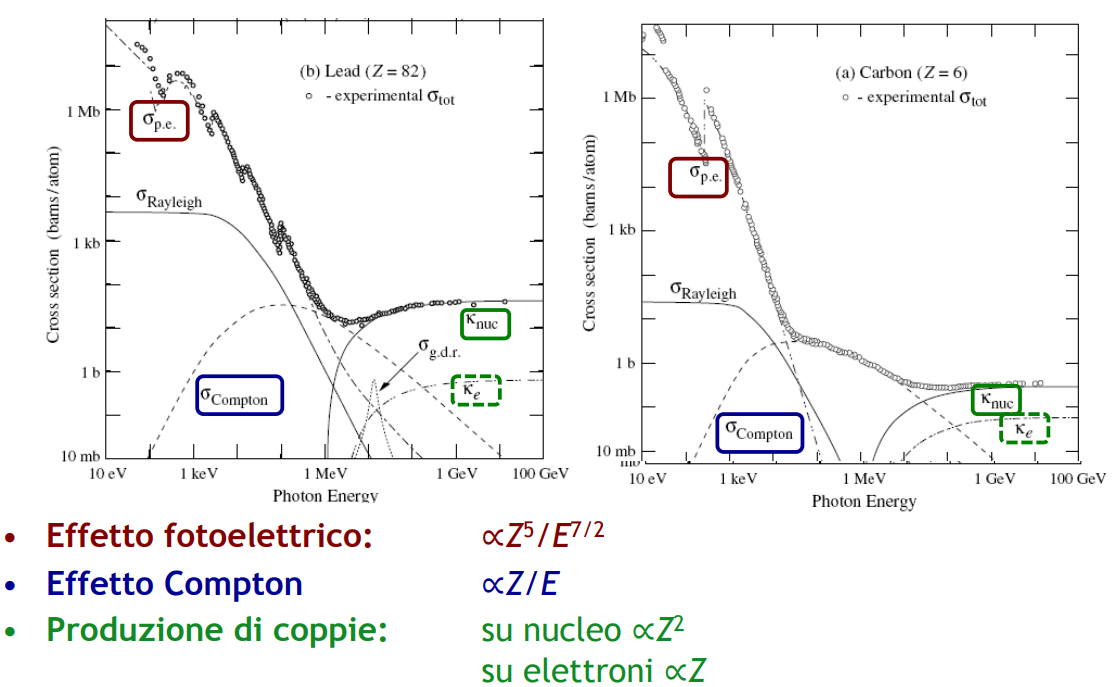
\includegraphics[scale=0.6]{Lezione14/h.png} 
\end{figure}
\subsection{Sciami elettromagnetici}
Un elettrone di "alta" energia perde energia principalmente per bremsstrahlung fin tanto che:
\begin{equation*}
    \left\langle\frac{dE}{dx}\right\rangle_{coll}<\frac{E}{X_0}
\end{equation*}
I fotoni prodotti possono convertirsi in coppie e gli elettroni/positroni prodotti irraggiano fotoni che possono convertirsi in coppie e così via. Così si sviluppa uno \textbf{sciame elettromagnetico}. Fino a quando vale la relazione sopra. Quando non vale più non ci sarà più produzione di fotoni e quindi questa catena si ferma.

\subsection{Sciami adronici}
La sezione d'urto per interazioni nucleari ad alta energia è proporzionale all'area del nucleo:
\begin{equation*}
    V_N\propto A\,\Rightarrow\,r_N\propto A^{1/3}\,\Rightarrow\,\sigma_N\approx\pi r_N^2\propto A^{2/3}
\end{equation*}
Il cammino libero per interazioni nucleari sarà:
\begin{equation*}
    \lambda_l=\frac{1}{n\sigma_N}=\frac{A}{\rho N_A\sigma_N}\propto\left(\frac{1}{\rho}\right)A^{1/3}
\end{equation*}
e prende il nome di lunghezza di interazione. In ogni interazioni possono venire prodotti adroni, i quali a loro volta possono interagire ecc ecc... \textbf{sciami adronici}. Attenzione! Gli adroni prodotti possono produrre $e^{\pm}$ o fotoni durante le interazioni e quindi la formazione degli sciami elettromagnetici secondari.
\subsection{Modello di Heitler degli sciami}
Sebbene adroni ed elettroni abbiano comportamenti diversi, possiamo stabilire un meccanismo generico per i processi di interazione tramite urti anelastici, da alcune semplici ipotesi: una particella percorre una lunghezza $\lambda$ tra un'interazione e l'altra; ad ogni interazione vengono prodotte $m$ particelle, con momento trasverso tipico $p_T$. Le particelle prodotte interagiscono a loro volta fino a quando l'energia non si è degradata sotto una certa energia critica $E_c$. a quel punto vengono semplicemente assorbite, in una distanza tipica $E_c/(dE/dx)_{coll}$. [slide]